% Digital Logic Report Template
% Created: 2020-01-10, John Miller

%==========================================================
%=========== Document Setup  ==============================

% Formatting defined by class file
\documentclass[11pt]{article}

% ---- Document formatting ----
\usepackage[margin=1in]{geometry}	% Narrower margins
\usepackage{booktabs}				% Nice formatting of tables
\usepackage{graphicx}				% Ability to include graphics

%\setlength\parindent{0pt}	% Do not indent first line of paragraphs 
\usepackage[parfill]{parskip}		% Line space b/w paragraphs
%	parfill option prevents last line of pgrph from being fully justified

% Parskip package adds too much space around titles, fix with this
\RequirePackage{titlesec}
\titlespacing\section{0pt}{8pt plus 4pt minus 2pt}{3pt plus 2pt minus 2pt}
\titlespacing\subsection{0pt}{4pt plus 4pt minus 2pt}{-2pt plus 2pt minus 2pt}
\titlespacing\subsubsection{0pt}{2pt plus 4pt minus 2pt}{-6pt plus 2pt minus 2pt}

% ---- Hyperlinks ----
\usepackage[colorlinks=true,urlcolor=blue]{hyperref}	% For URL's. Automatically links internal references.

% ---- Code listings ----
\usepackage{listings} 					% Nice code layout and inclusion
\usepackage[usenames,dvipsnames]{xcolor}	% Colors (needs to be defined before using colors)

% Define custom colors for listings
\definecolor{listinggray}{gray}{0.98}		% Listings background color
\definecolor{rulegray}{gray}{0.7}			% Listings rule/frame color

% Style for Verilog
\lstdefinestyle{Verilog}{
	language=Verilog,					% Verilog
	backgroundcolor=\color{listinggray},	% light gray background
	rulecolor=\color{blue}, 			% blue frame lines
	frame=tb,							% lines above & below
	linewidth=\columnwidth, 			% set line width
	basicstyle=\small\ttfamily,	% basic font style that is used for the code	
	breaklines=true, 					% allow breaking across columns/pages
	tabsize=3,							% set tab size
	commentstyle=\color{gray},	% comments in italic 
	stringstyle=\upshape,				% strings are printed in normal font
	showspaces=false,					% don't underscore spaces
}

% How to use: \Verilog[listing_options]{file}
\newcommand{\Verilog}[2][]{%
	\lstinputlisting[style=Verilog,#1]{#2}
}




%======================================================
%=========== Body  ====================================
\begin{document}

\title{ELC 2137 Lab 9: ALU with input register}
\author{Alexander Noll}

\maketitle


\section*{Summary}

In the lab, two D register memory units and an Arithmetic Logic Unit (ALU)  were created. Using a mixture of sequential and combinational logic in Verilog, the Basys3 board was programed to add, subtract, and compare two numbers. The comparisons were done bitwise using AND, OR, and XOR gates.



\section*{Results}

\begin{table*}[ht]\centering
	\caption{\textit{register} expected results table}
	\label{ALU:tbl:register_ERT}\medskip
	\begin{tabular}{l|rrrrrrrrrrr}
		Time (ns): & 0-5 & 5-10 & 10-15 & 15-20 & 20-25 & 25-30 & 30-35 & 35-40 & 40-45 & 45-50 & 50-55 \\
		\midrule
		D (hex) & 0 & 0 	  & A & A & 3 	    & 3 	  & 0 	    & 0 & 0$\to$6 & 6 & 6 \\
		clk     & 0 & 1 	  & 0 & 1 & 0 	    & 1 	  & 0 	    & 1 & 0 	  & 1 & 0 \\
		en  	& 0 & 0 	  & 1 & 1 & 1$\to$0 & 0$\to$1 & 1$\to$0 & 0 & 0$\to$1 & 1 & 1 \\
		rst 	& 0 & 0$\to$1 & 0 & 0 & 0 		& 0 	  & 0		& 0 & 0		  & 0 & 0 \\
		\midrule
		Q (hex) & X & X$\to$0 & 0 & A & A & A & A & A & A & 6 & 6\\
		\bottomrule
	\end{tabular}
\end{table*}

\begin{figure}[ht]\centering
	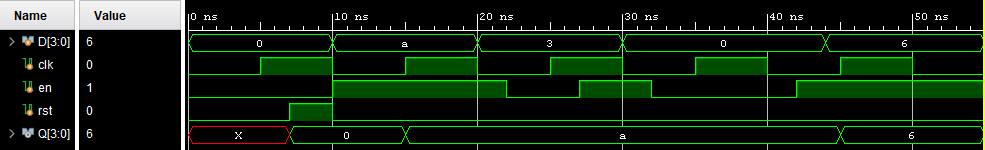
\includegraphics[width=1.0\textwidth,trim=0 0mm 0 0,clip]{RegisterTest}
	\caption{Register Test Waveform}
\end{figure}

\begin{table*}[ht]\centering
	\caption{\textit{alu} expected results table skeleton}
	\label{ALU:tbl:alu_ERT}\medskip
	\begin{tabular}{l|rrrrr}
		Time (ns): & 0-5 & 5-10 & 10-15 & 15-20 & 20-25 \\
		\midrule
		in0 & 0C & 0C & 0C & 0C & 0C \\
		in1 & 07 & 07 & 07 & 07 & 07 \\
		op	& 0 & 1 & 2 & 3 & 4  \\
		\midrule
		out & 13 & 05 & 04 & 0F & 0D	  \\
		\bottomrule
	\end{tabular}
\end{table*}

\begin{figure}[ht]\centering
	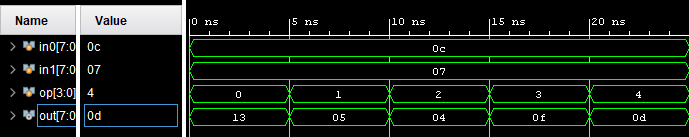
\includegraphics[width=1.0\textwidth,trim=0 0mm 0 0,clip]{ALUTest}
	\caption{ALU Test Waveform}
\end{figure}

\begin{figure}[ht]\centering
	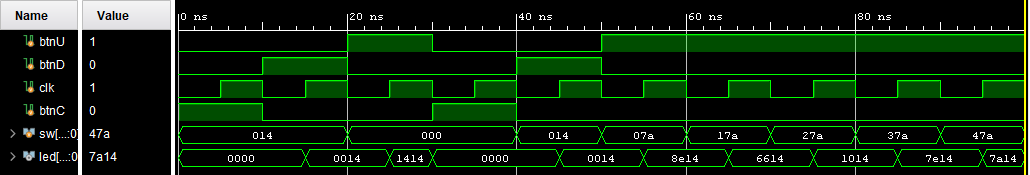
\includegraphics[width=1.0\textwidth,trim=0 0mm 0 0,clip]{basys3_lab9}
	\caption{Top Lab 9 Test Waveform}
\end{figure}

\begin{figure}[ht]\centering
	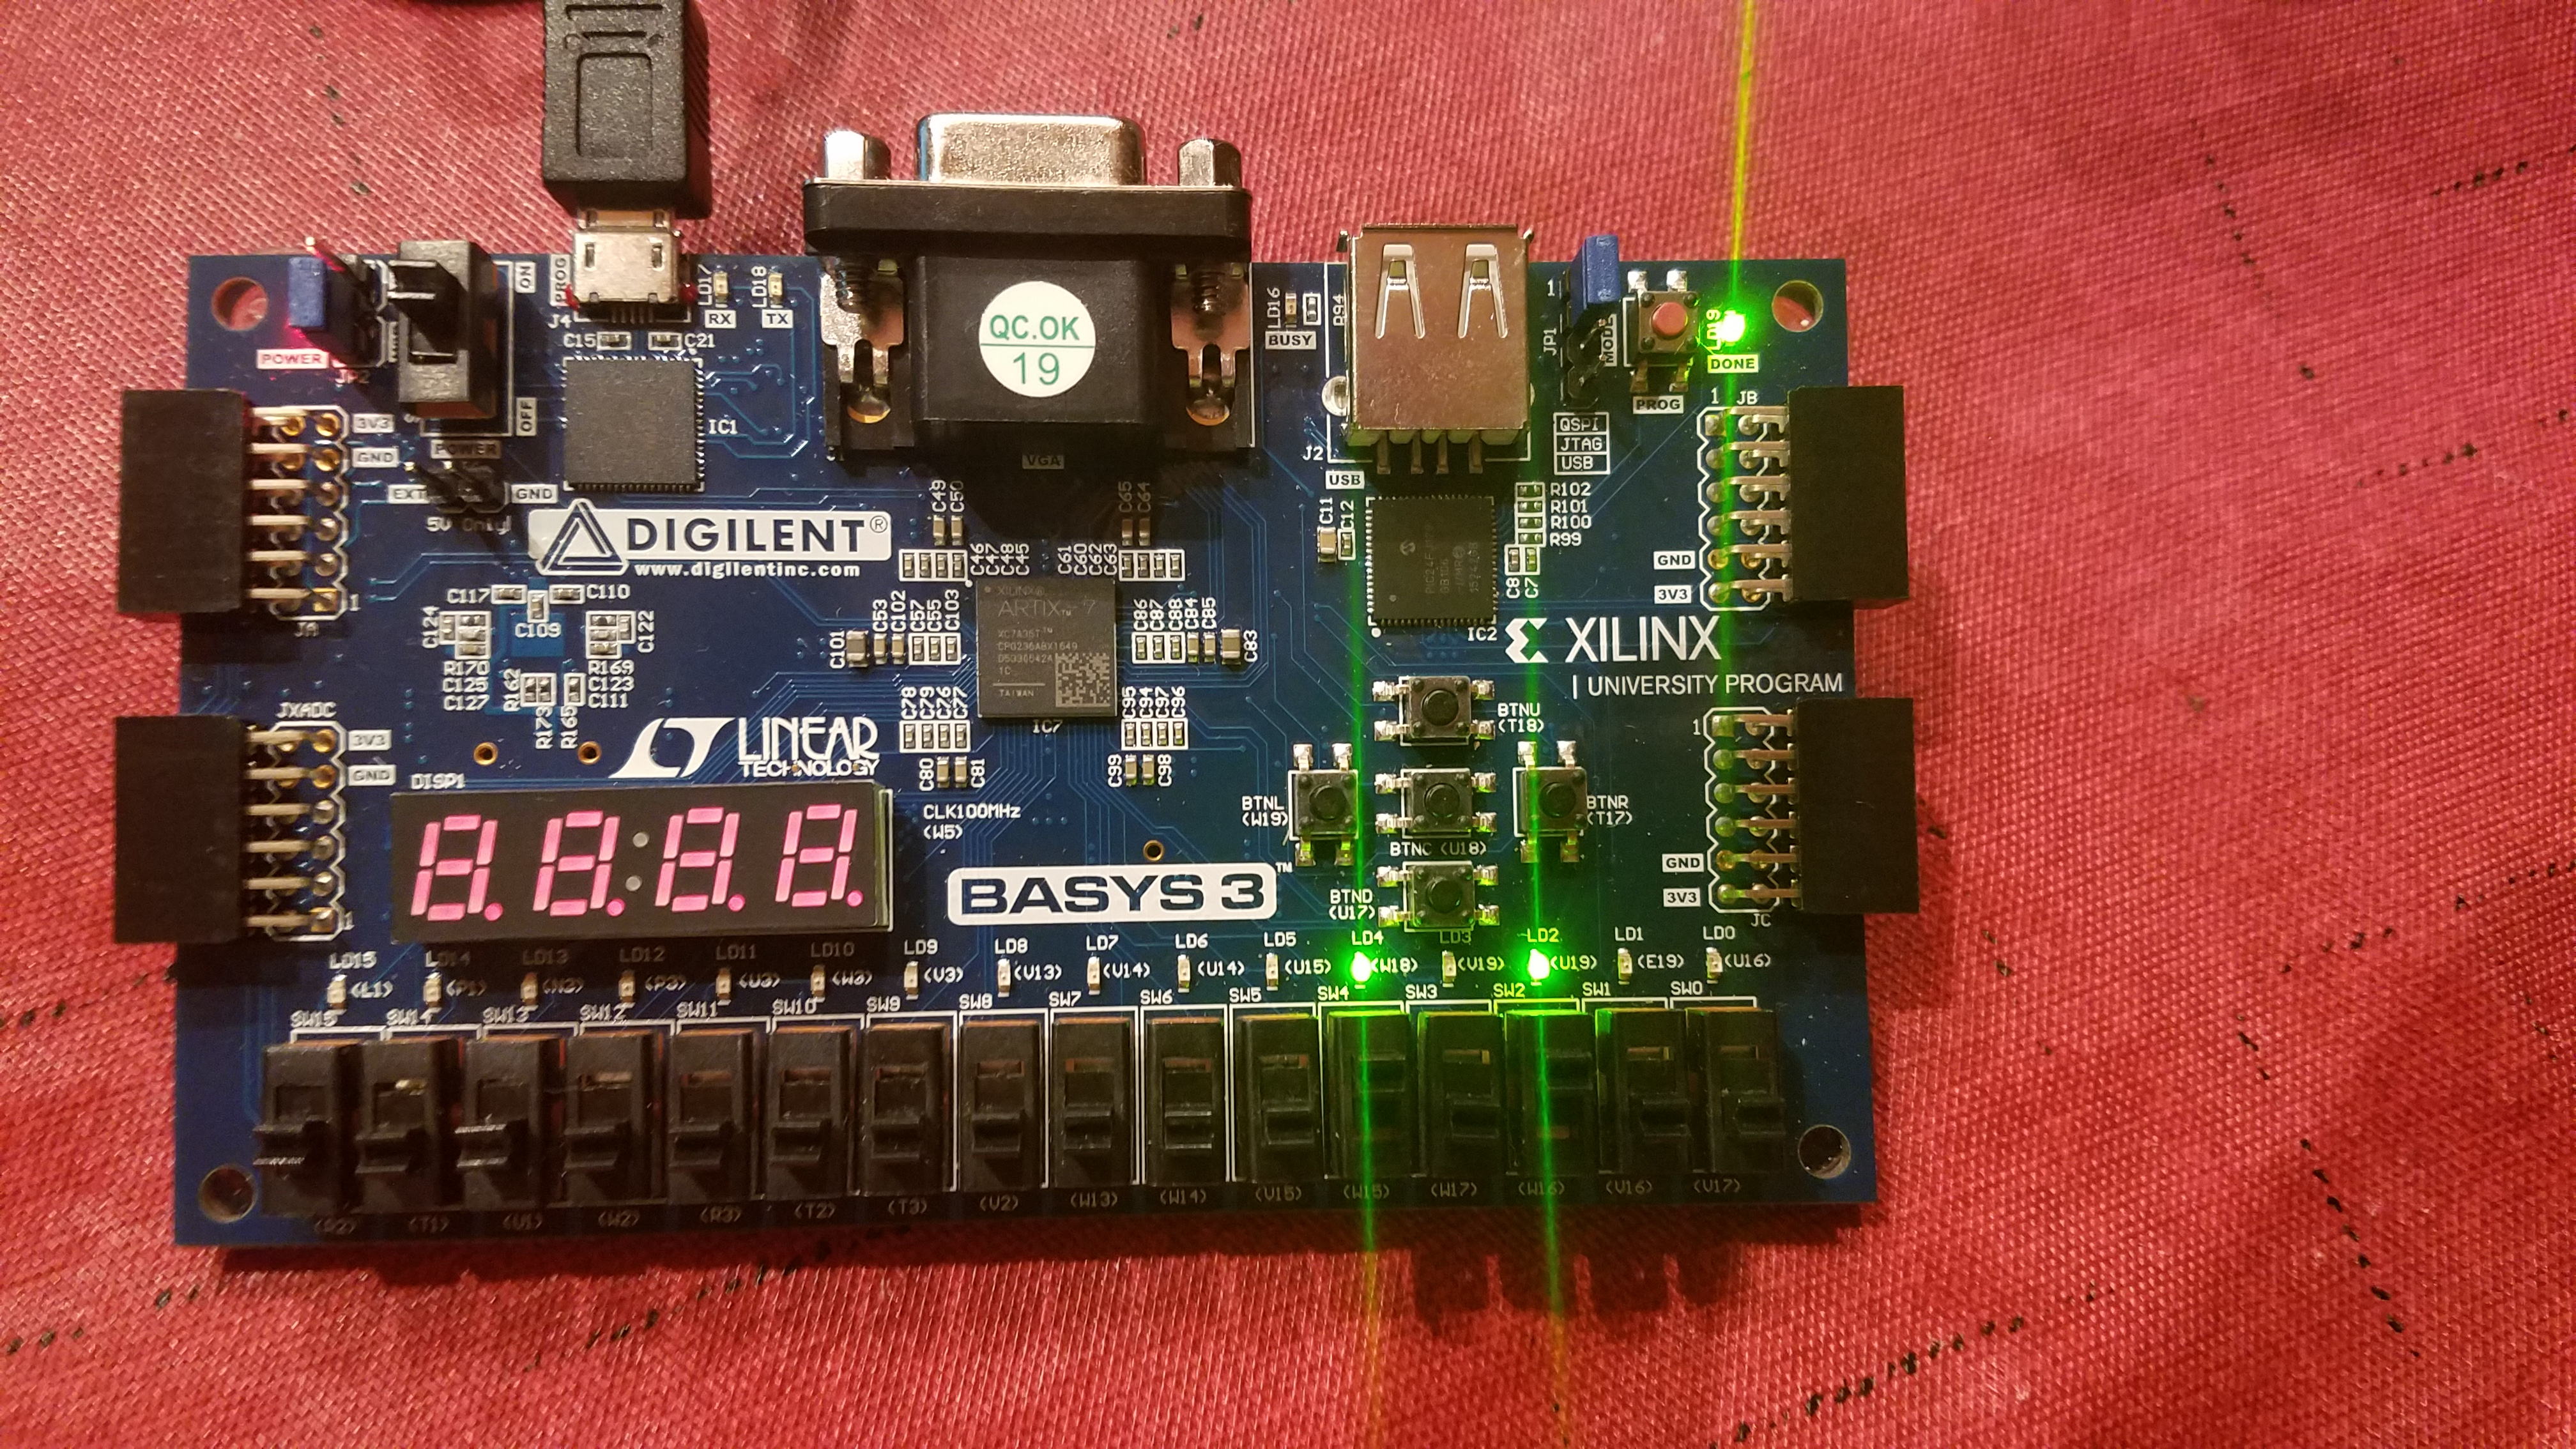
\includegraphics[width=1.0\textwidth,trim=0 10mm 0 0,clip]{Step1}
	\caption{Board Operation Step 1}
\end{figure}

\begin{figure}[ht]\centering
	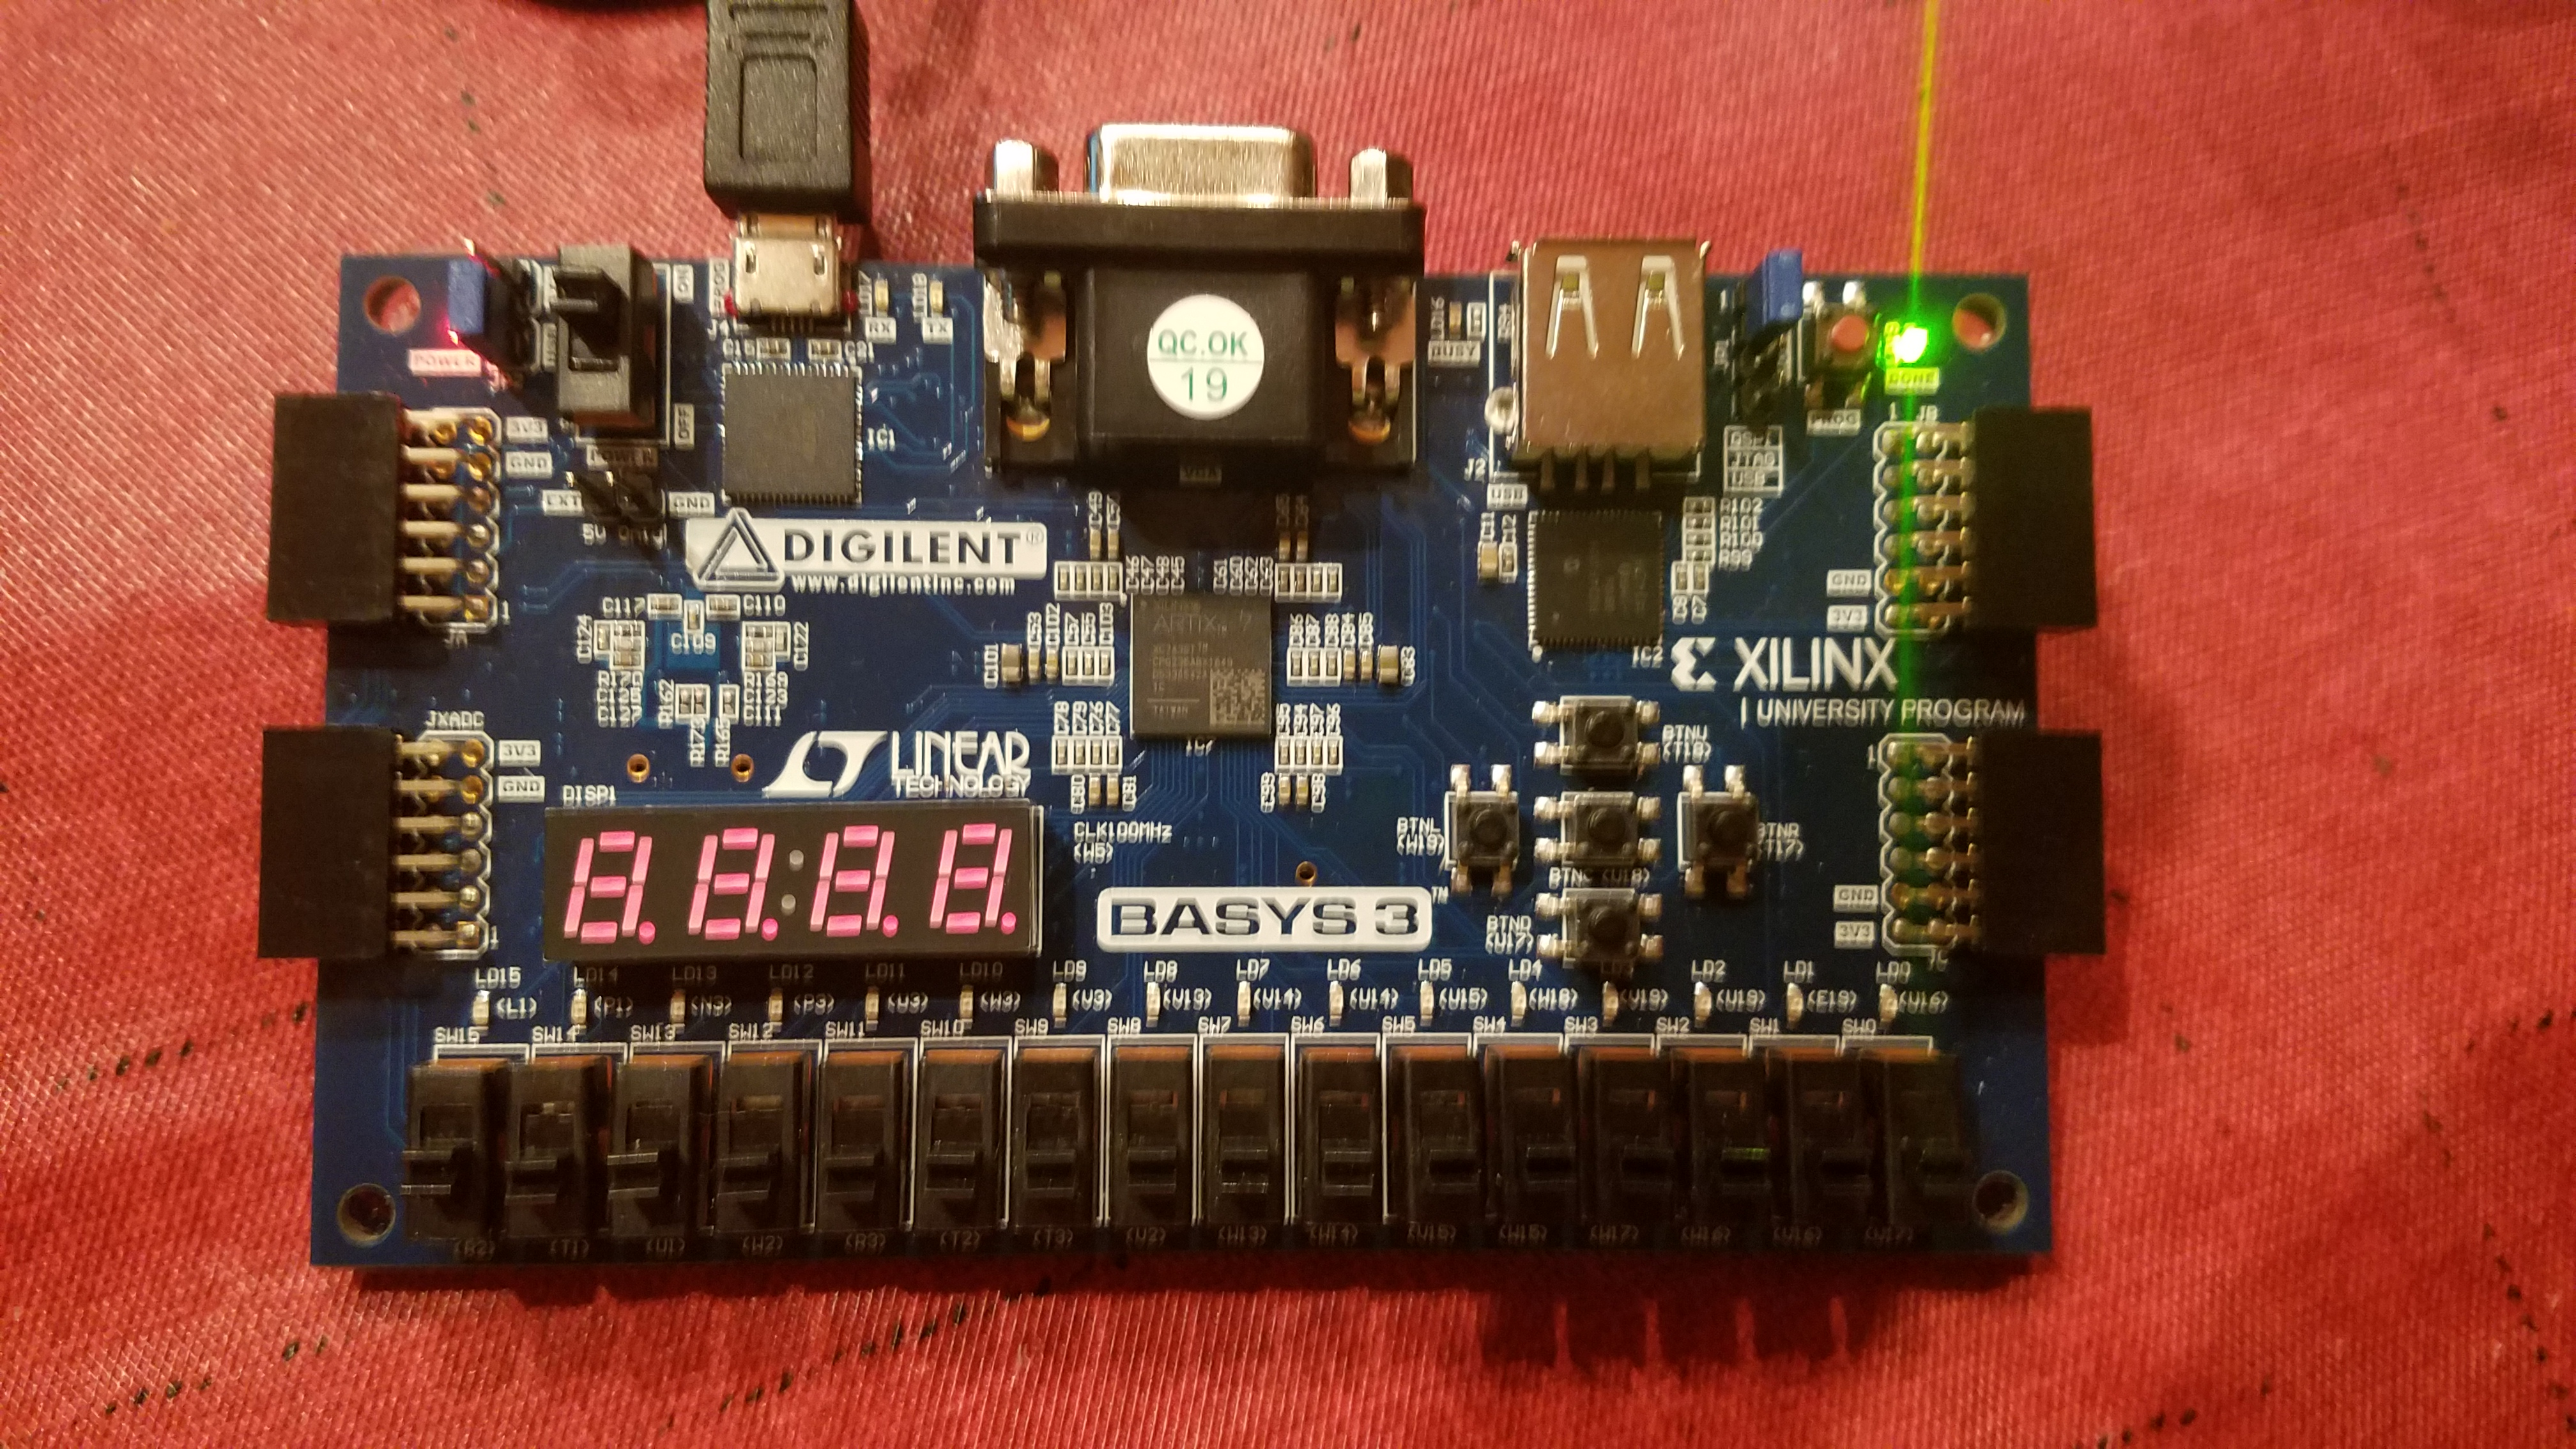
\includegraphics[width=1.0\textwidth,trim=0 0mm 0 0,clip]{Step3}
	\caption{Board Operation Step 2}
\end{figure}

\begin{figure}[ht]\centering
	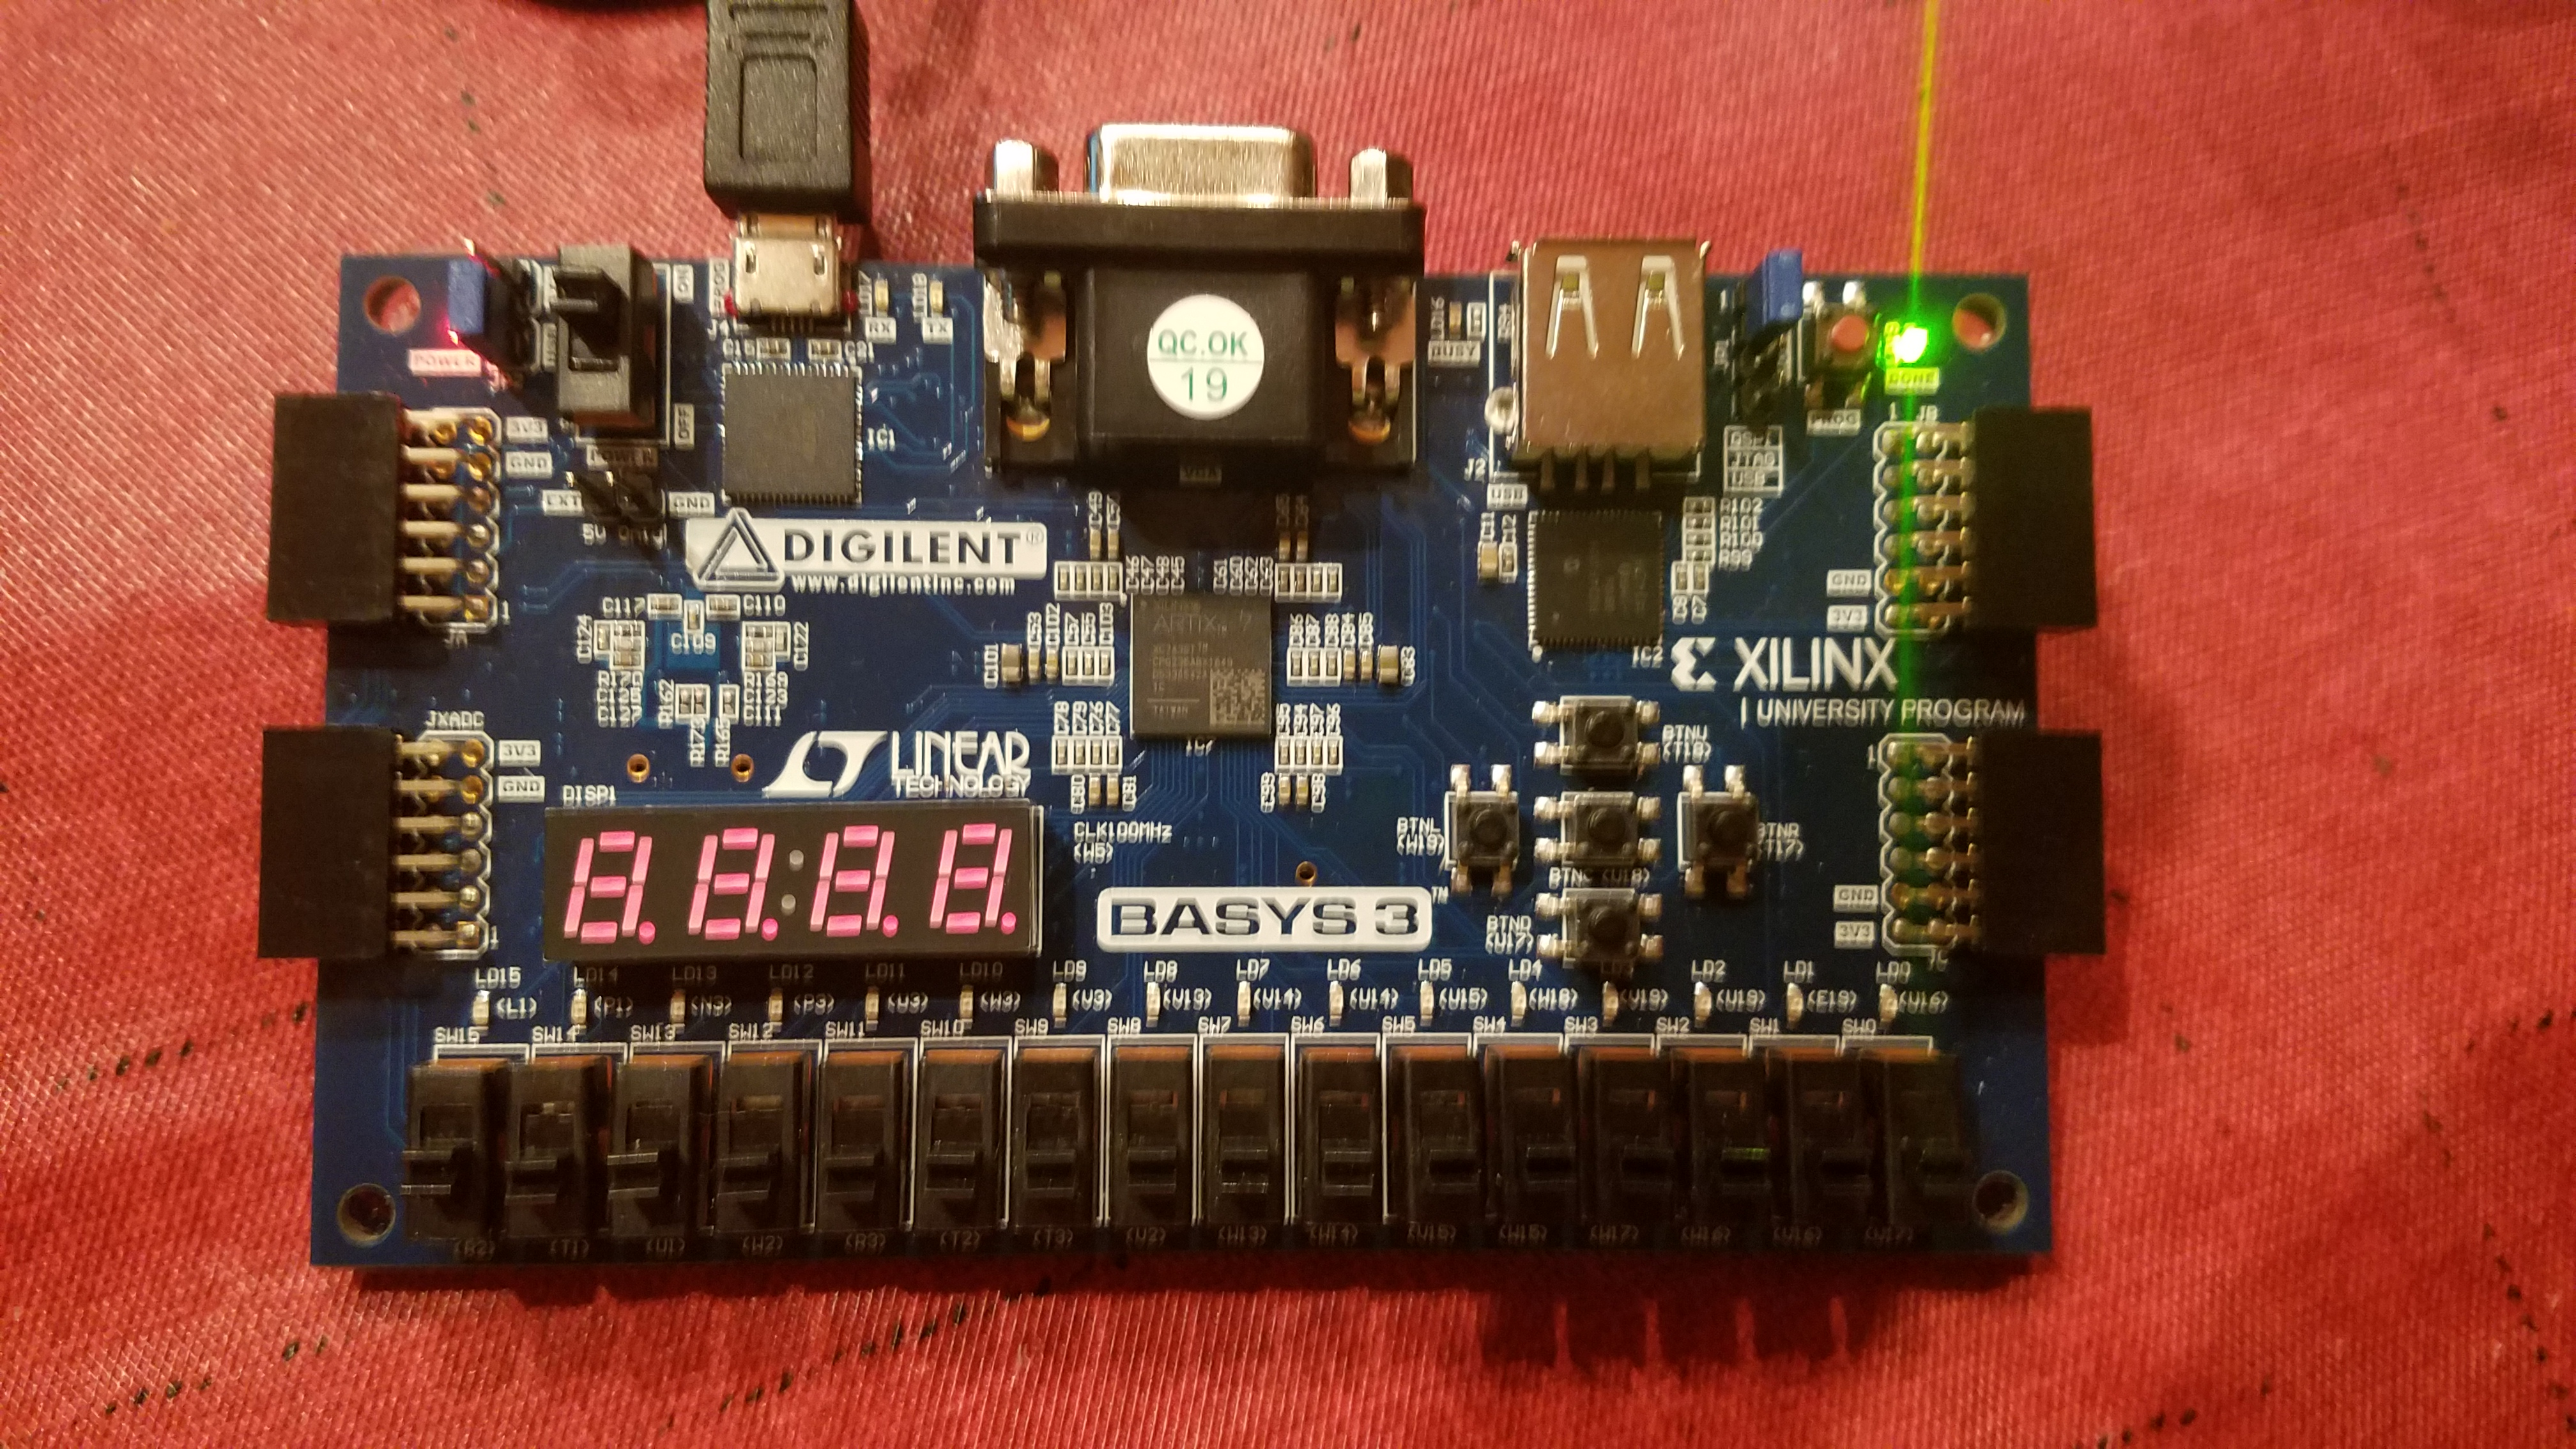
\includegraphics[width=1.0\textwidth,trim=0 0mm 0 0,clip]{Step3}
	\caption{Board Operation Step 3}
\end{figure}

\begin{figure}[ht]\centering
	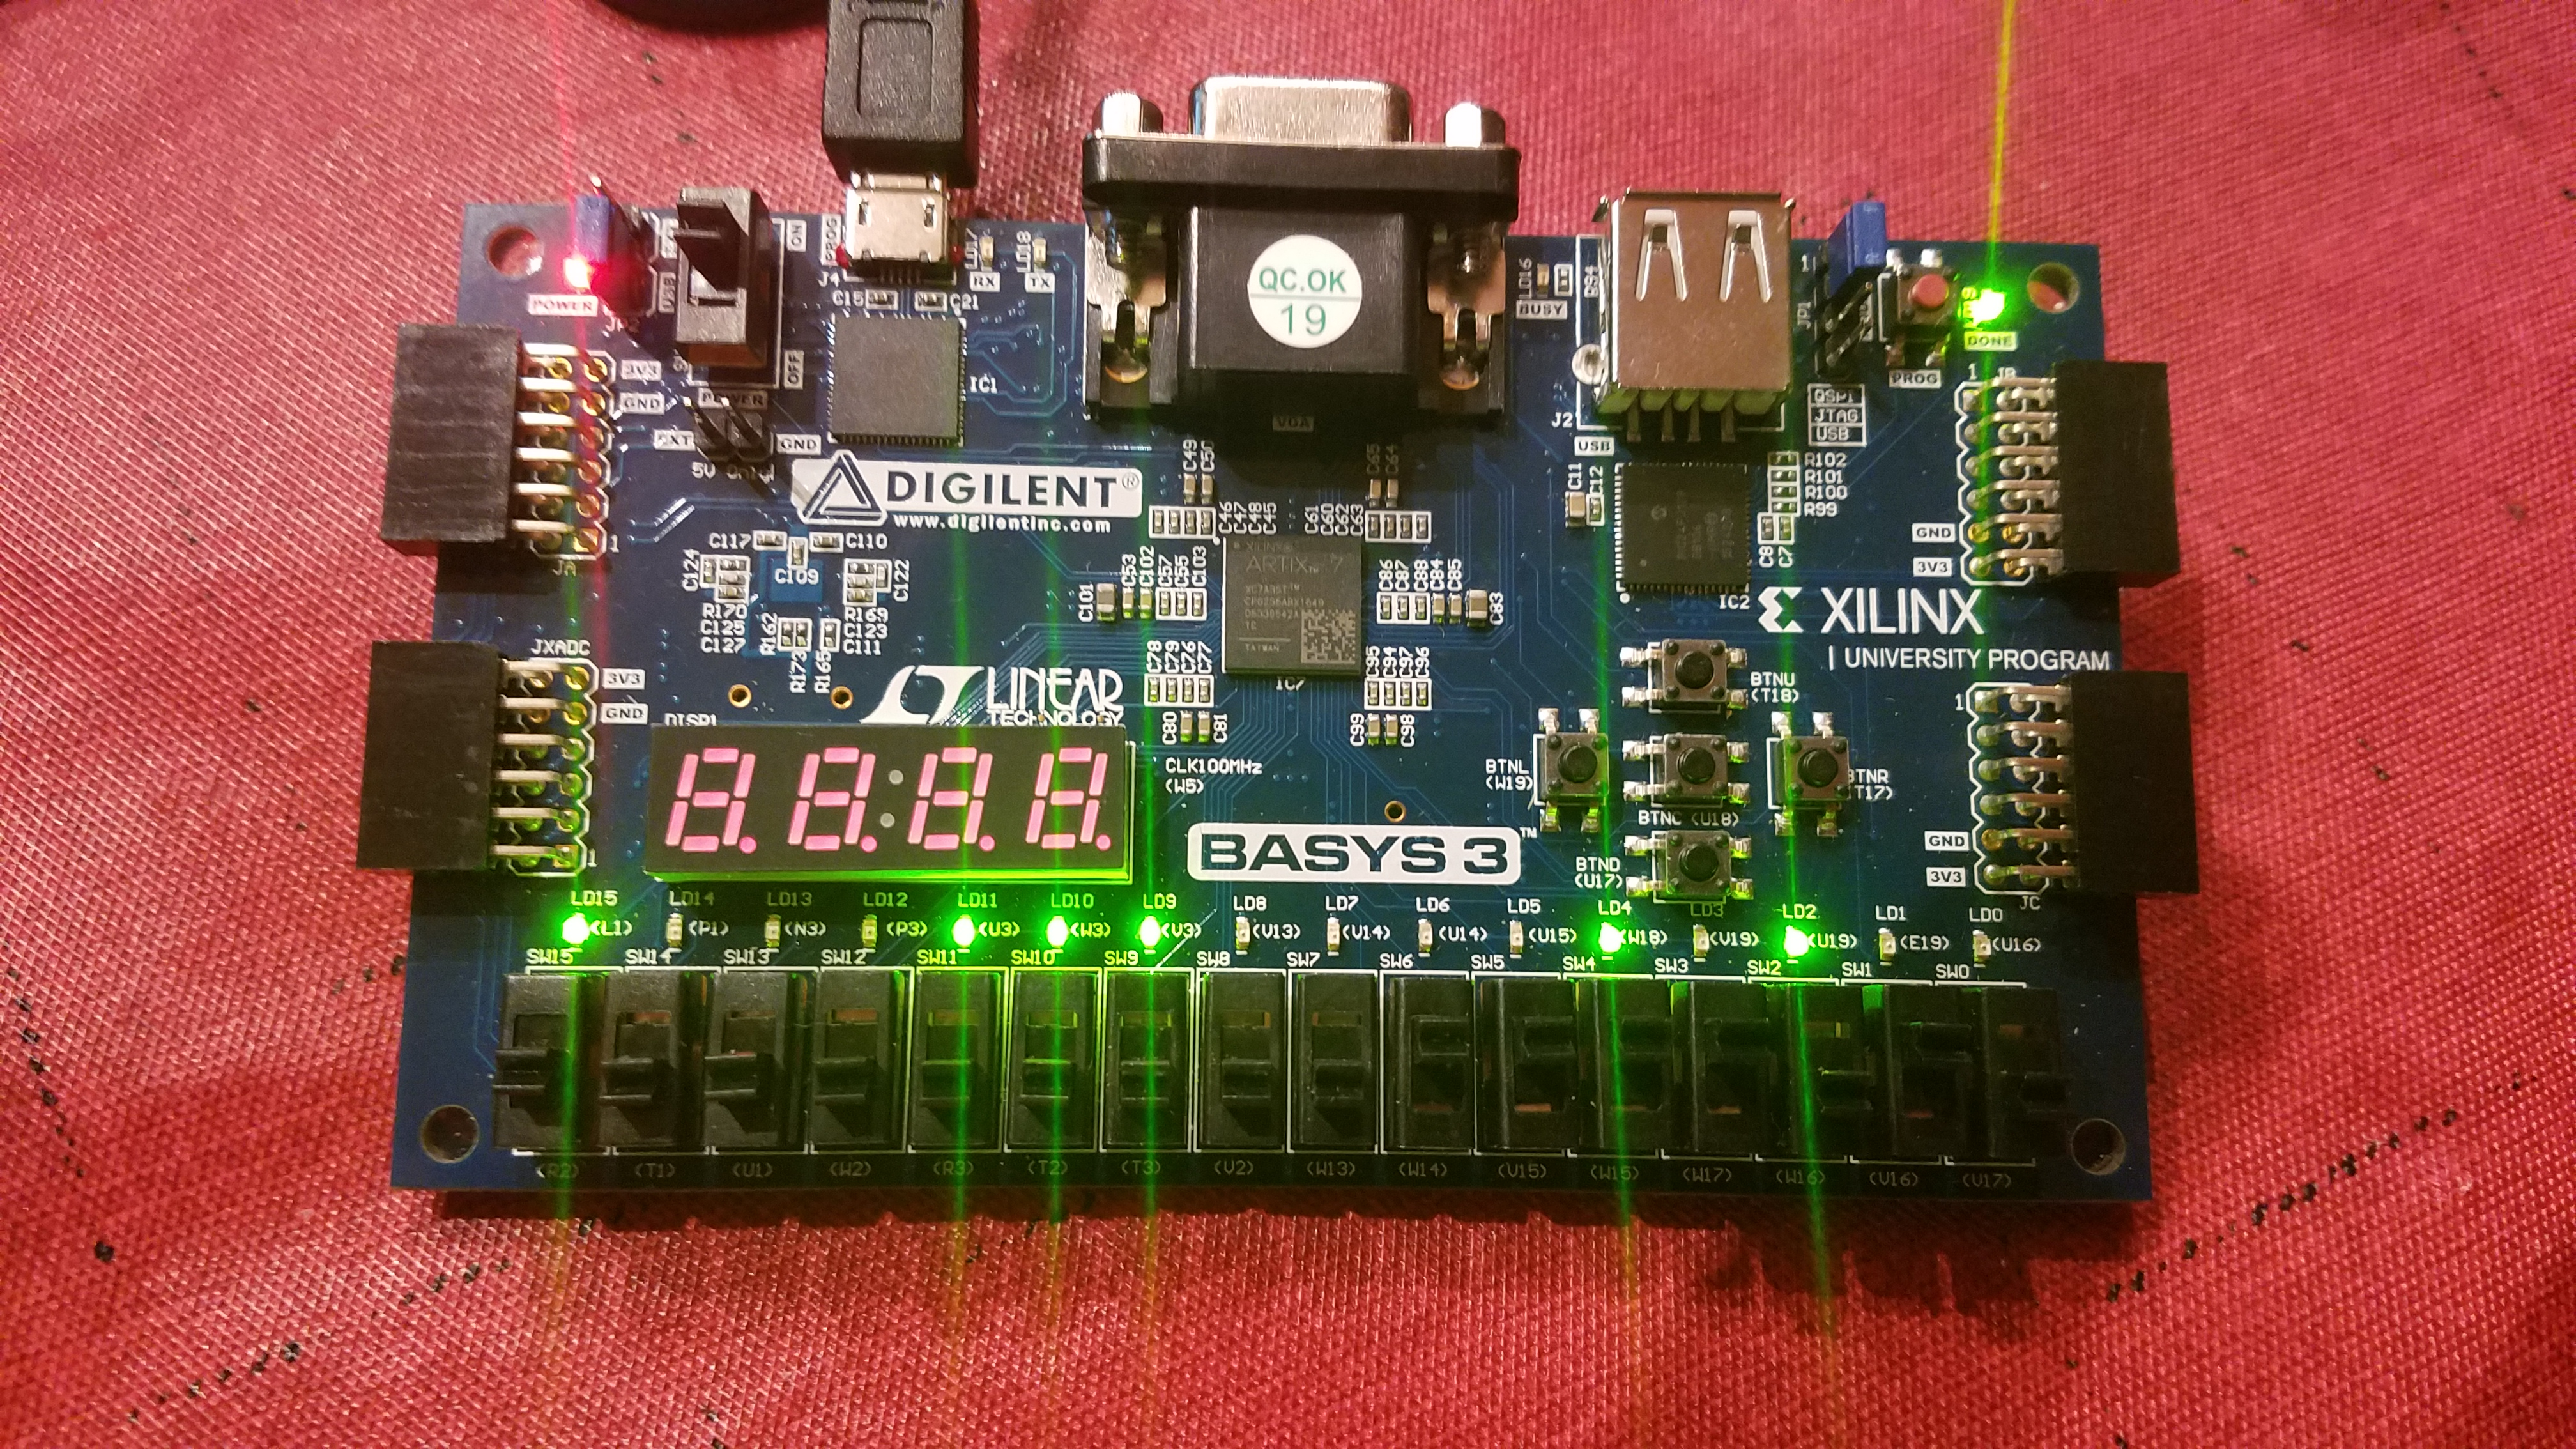
\includegraphics[width=1.0\textwidth,trim=0 0mm 0 0,clip]{Step4}
	\caption{Board Operation Step 4- Operation 0(Add)}
\end{figure}

\begin{figure}[ht]\centering
	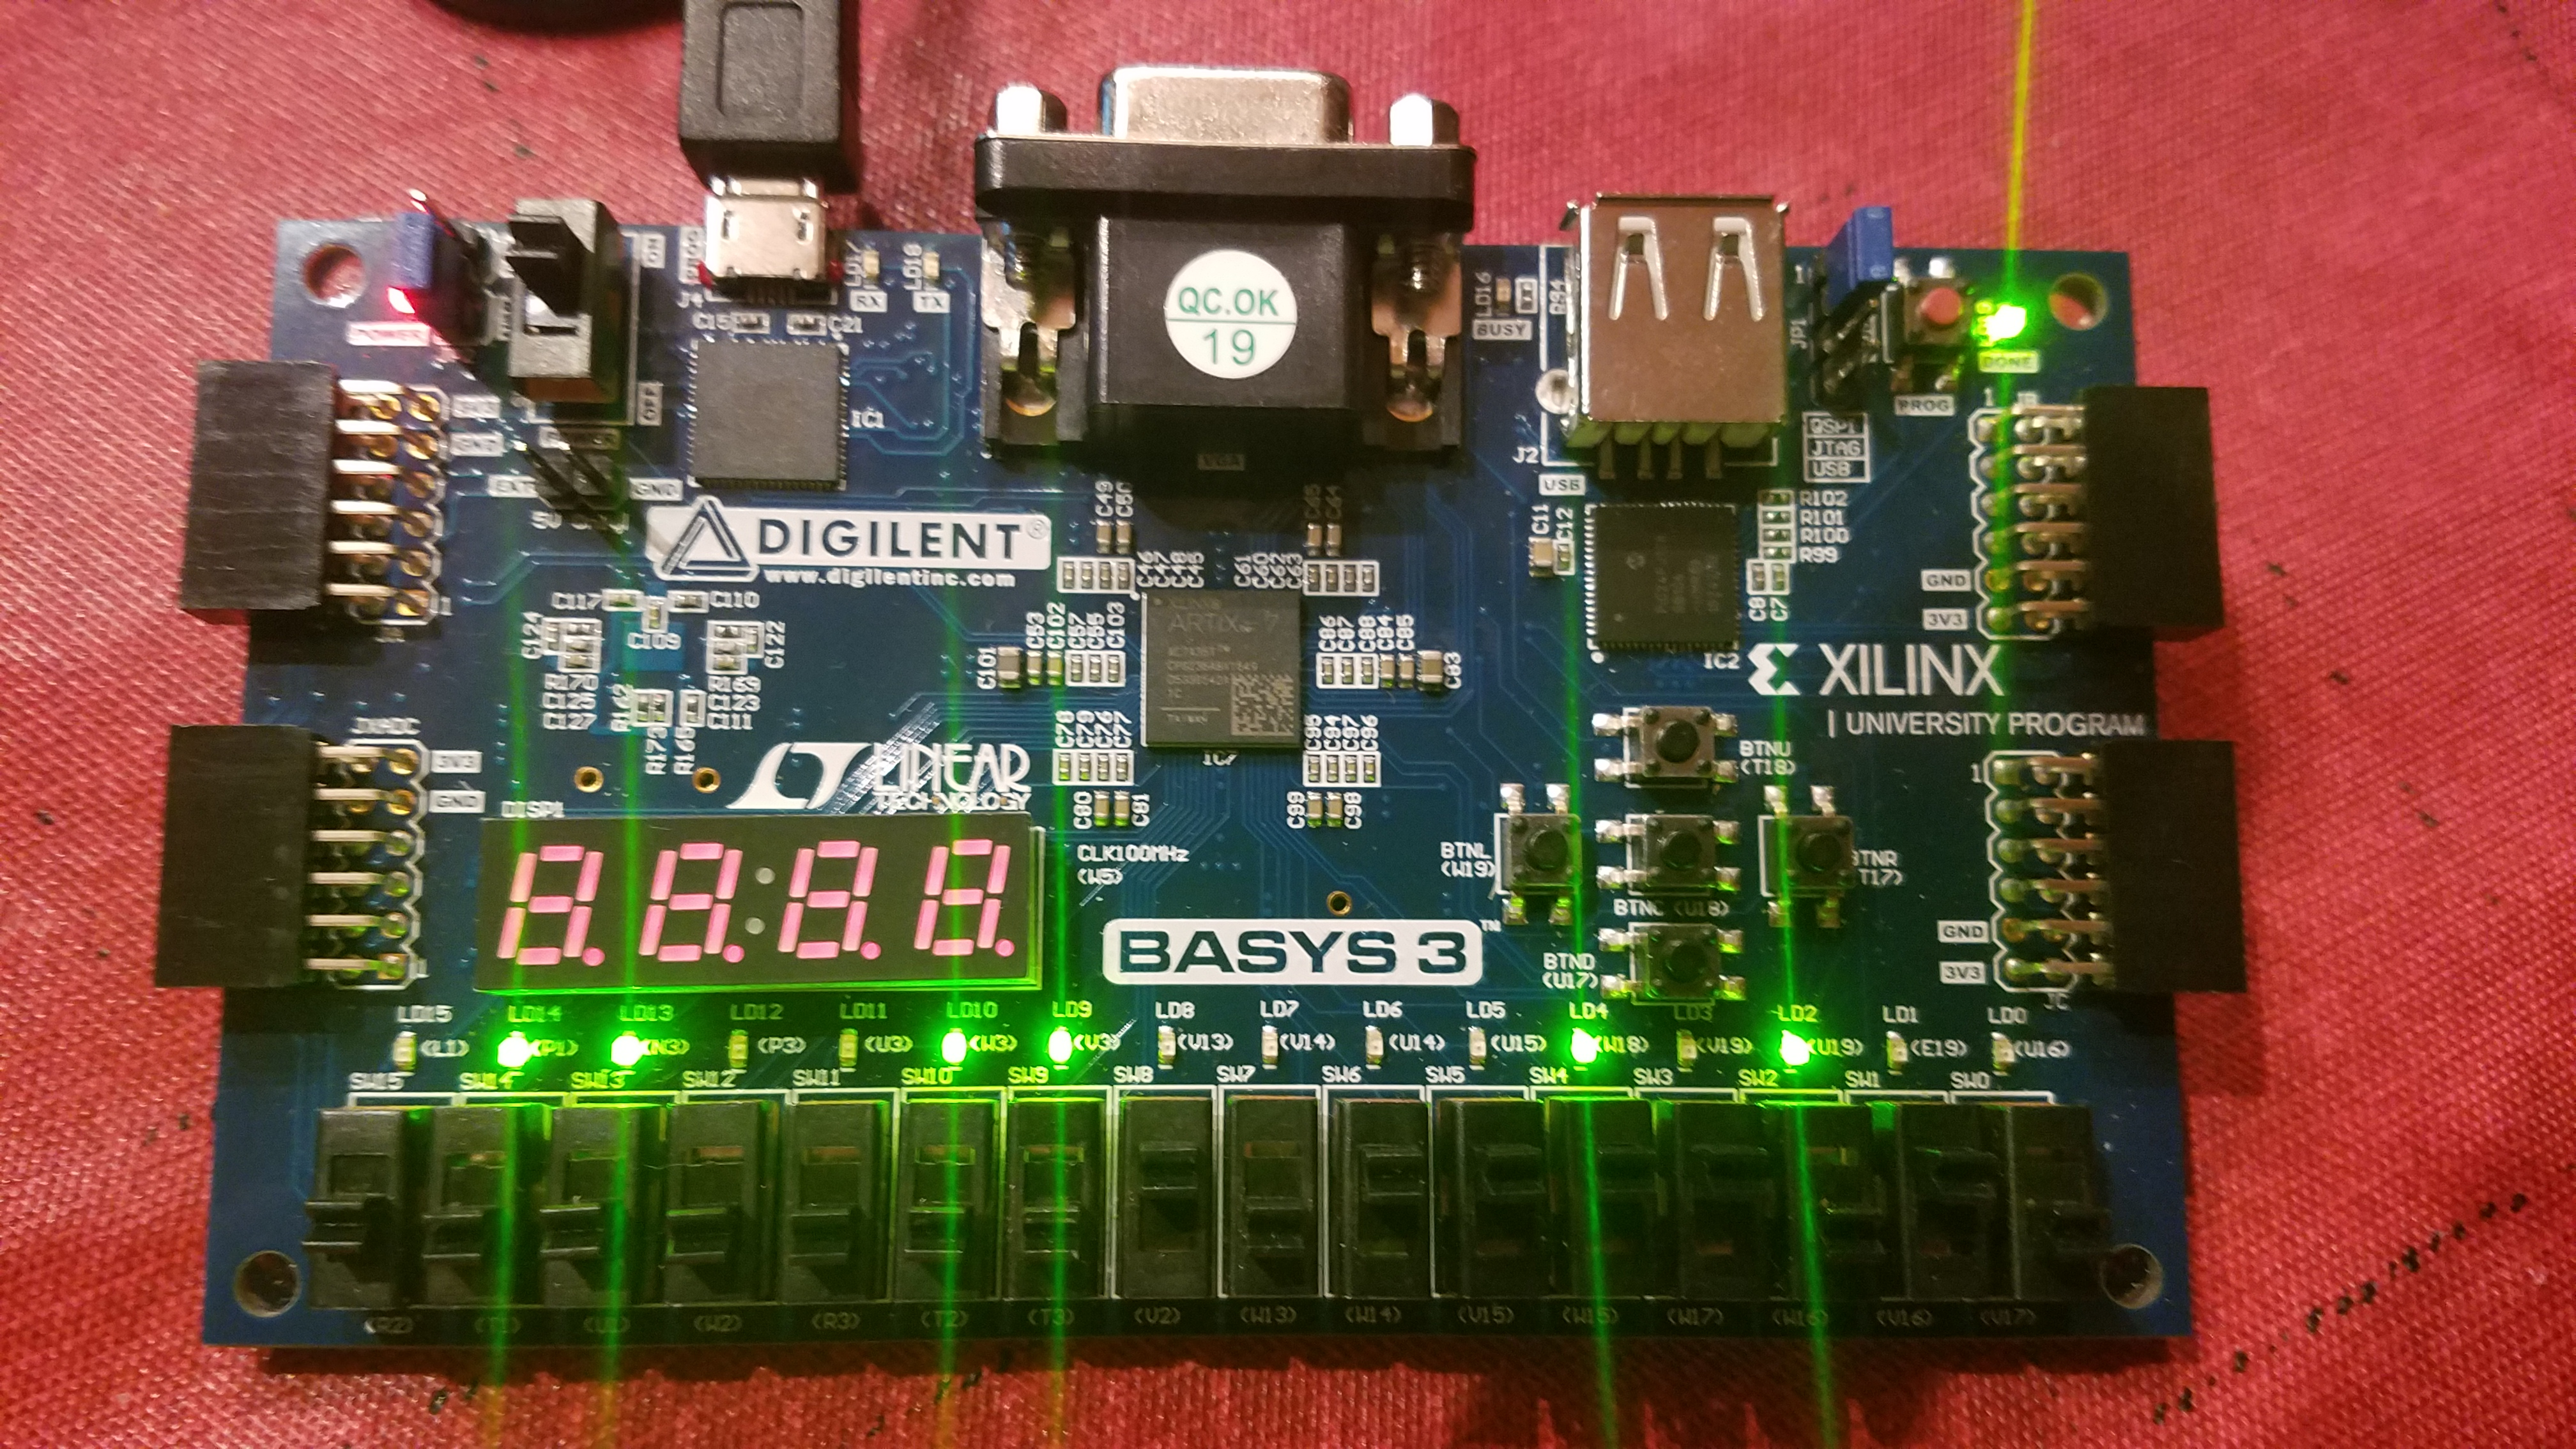
\includegraphics[width=1.0\textwidth,trim=0 0mm 0 0,clip]{Op1}
	\caption{Board Operation Step 5 -Operation 1(Subtract)}
\end{figure}

\begin{figure}[ht]\centering
	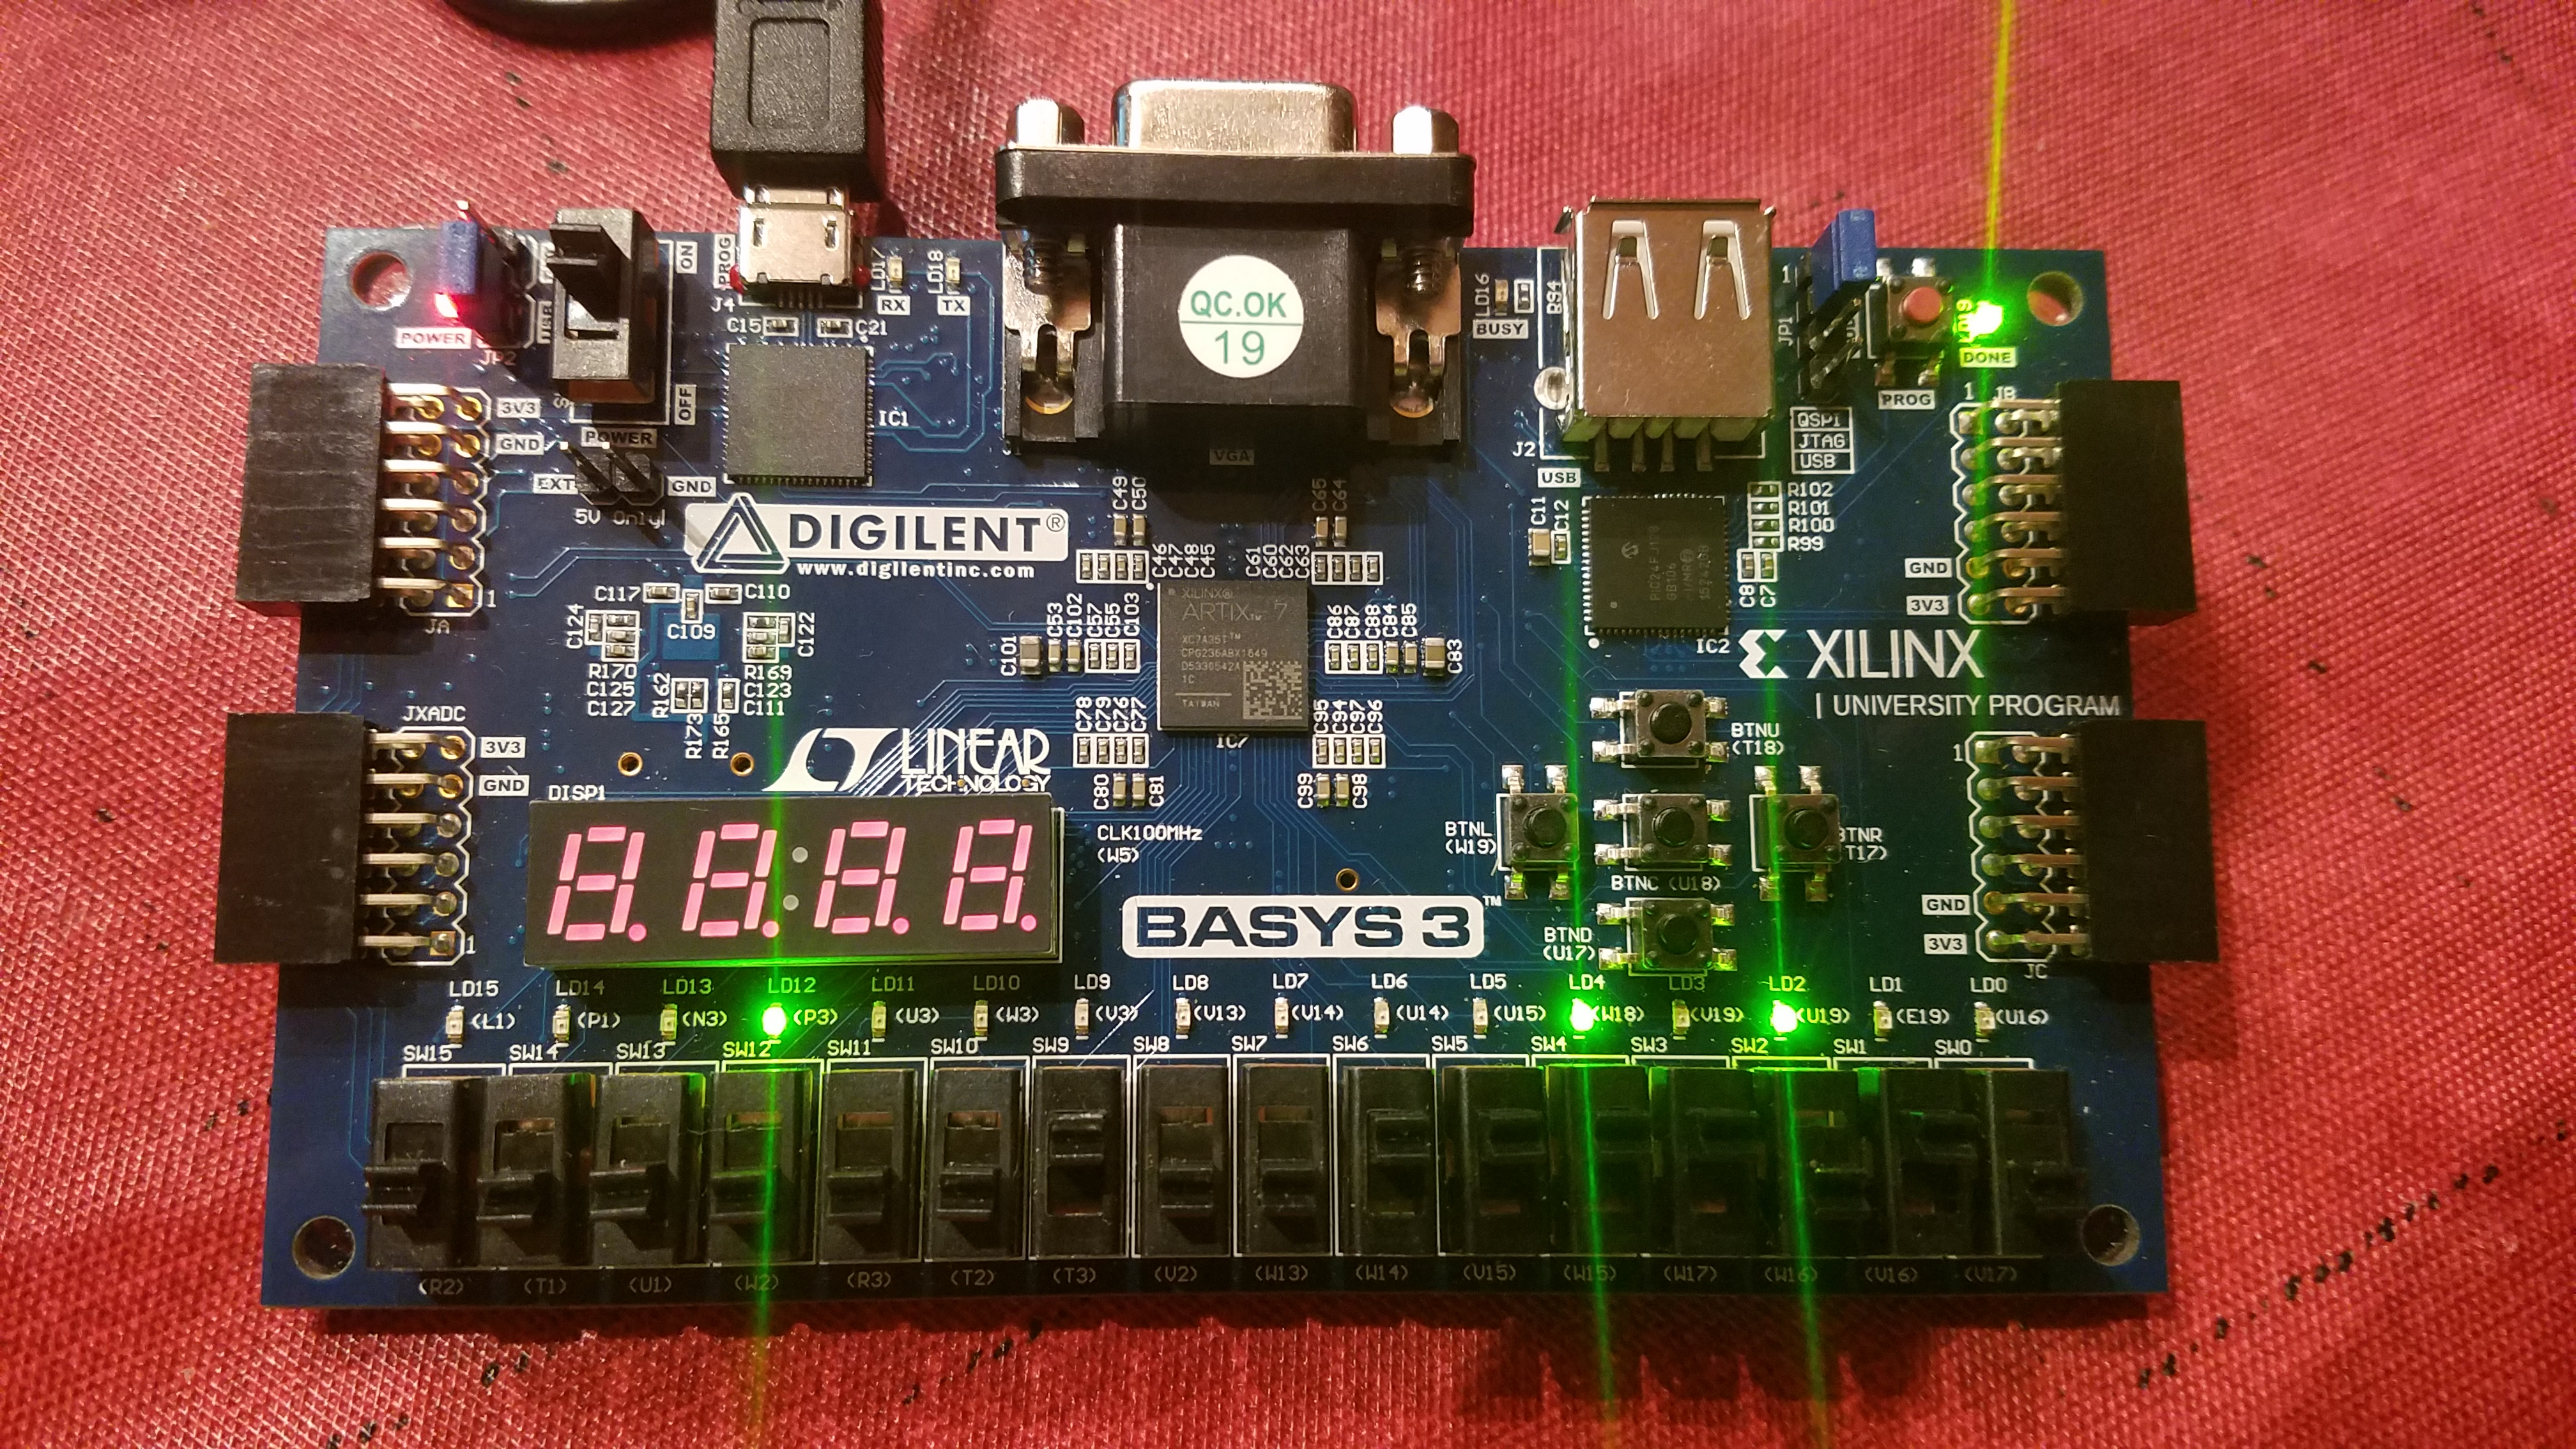
\includegraphics[width=1.0\textwidth,trim=0 0mm 0 0,clip]{Op2}
	\caption{Board Operation Step 6 -Operation 2(AND)}
\end{figure}

\begin{figure}[ht]\centering
	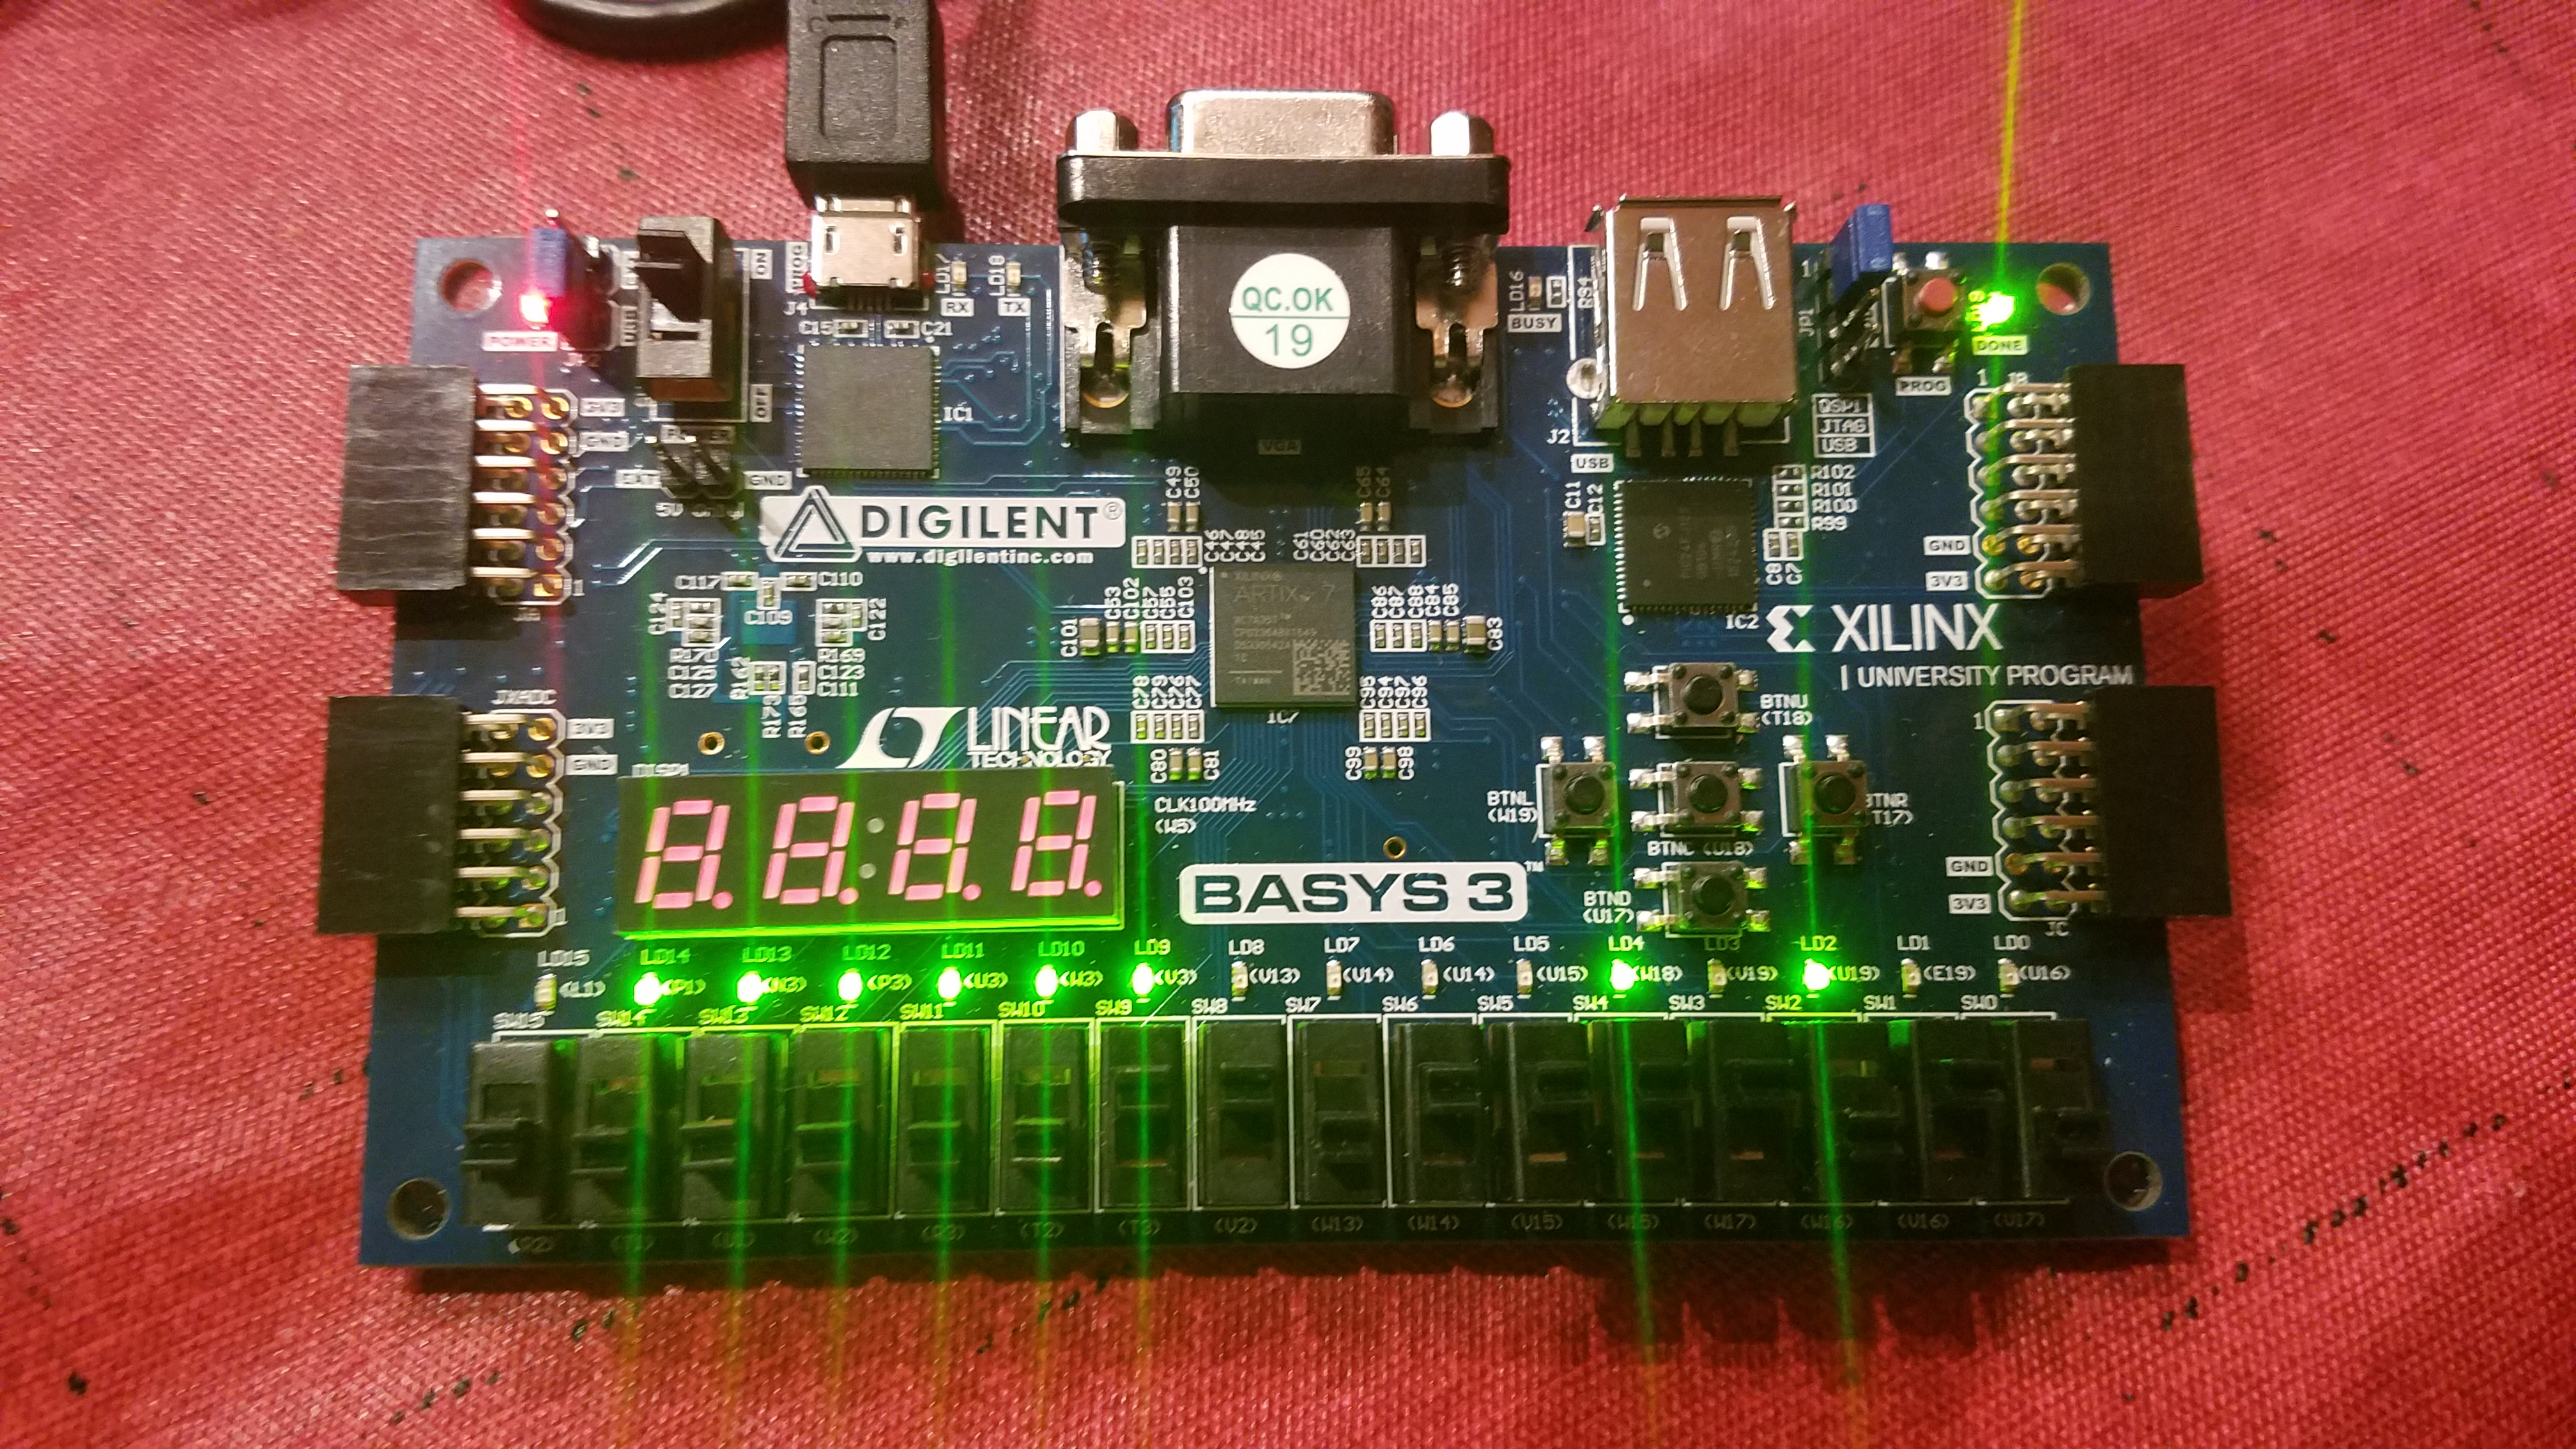
\includegraphics[width=1.0\textwidth,trim=0 0mm 0 0,clip]{Op3}
	\caption{Board Operation Step 7 -Operation 3(OR)}
\end{figure}

\begin{figure}[ht]\centering
	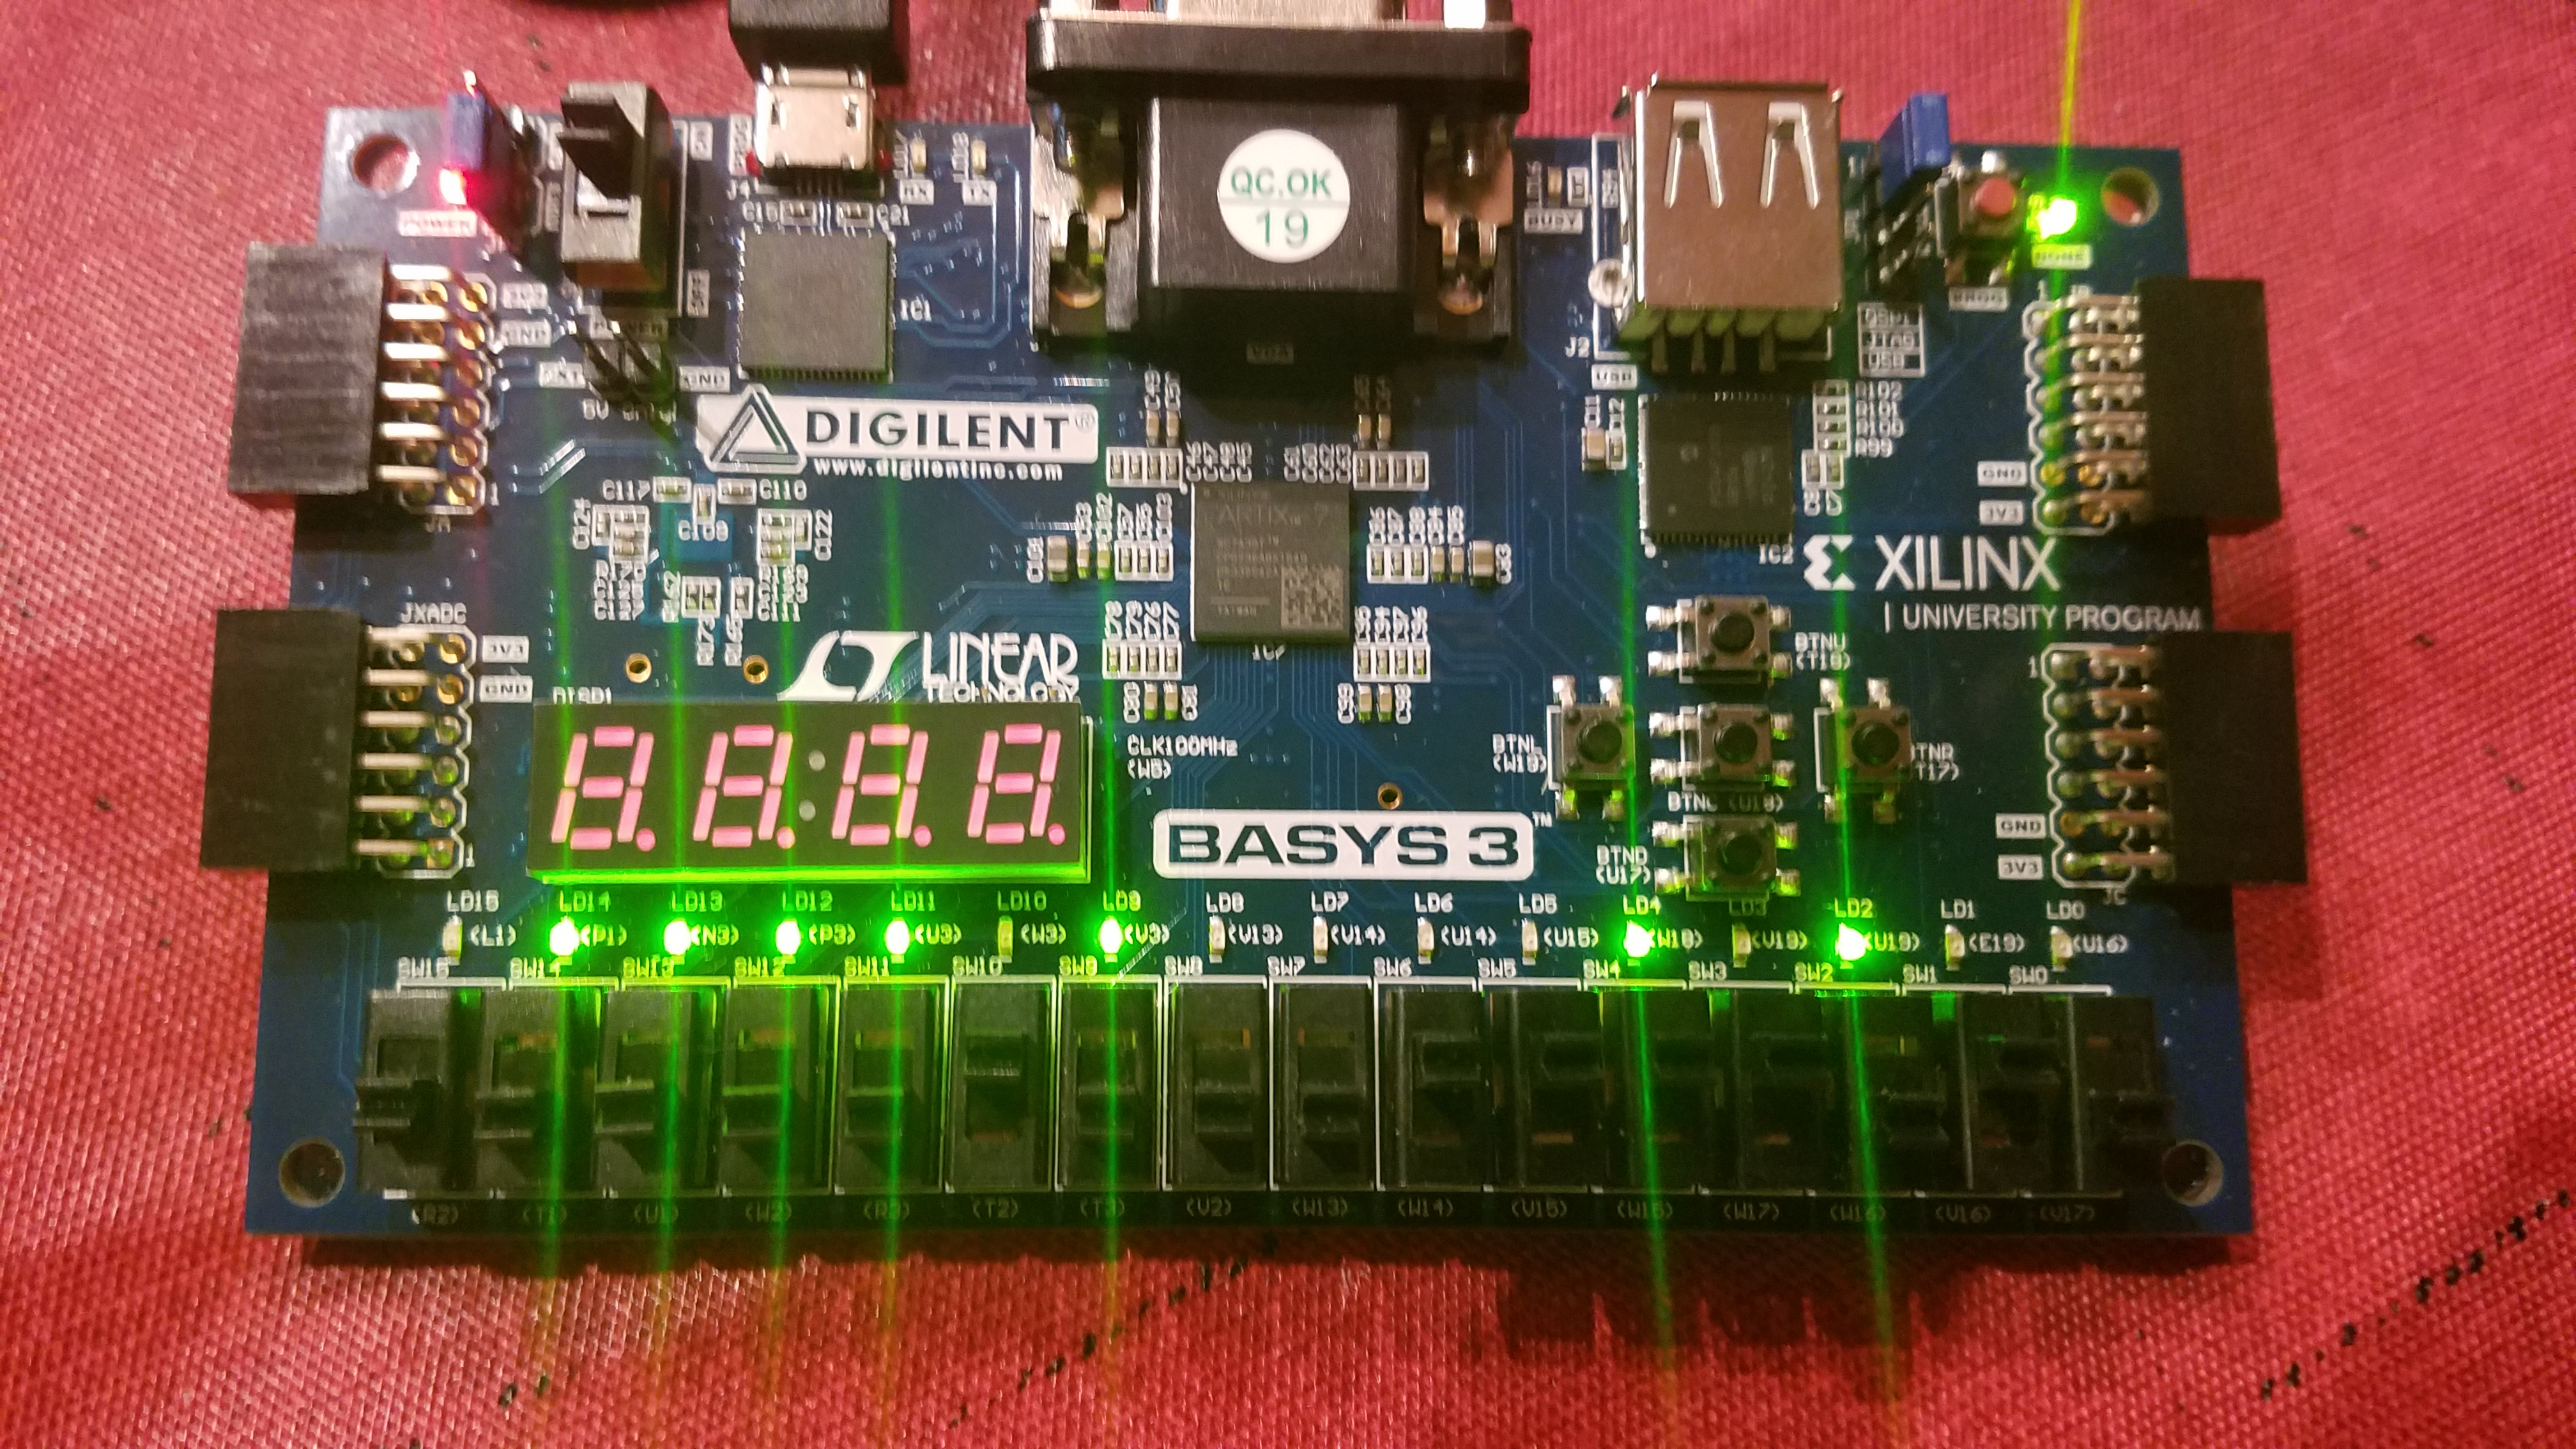
\includegraphics[width=1.0\textwidth,trim=0 0mm 0 0,clip]{Op4}
	\caption{Board Operation Step 8 -Operation 4(XOR)}
\end{figure}


	\clearpage

\section*{Code}

\Verilog[firstline=23, lastline=43,caption=Verilog Register Source,label=code:file_ex]
{register.sv}

\Verilog[firstline=23, lastline=48,caption=Verilog ALU Source,label=code:file_ex]
{alu.sv}

\Verilog[firstline=23, lastline=35,caption=Verilog Top Lab 9 Source,label=code:file_ex]
{top_lab9.sv}

\Verilog[firstline=23, lastline=48,caption=Verilog register Test Bench,label=code:file_ex]
{register_test.sv}

\clearpage

\Verilog[firstline=23, lastline=43,caption=Verilog ALU Test Bench,label=code:file_ex]
{alu_test.sv}



\end{document}
